\documentclass[11pt]{article}
\usepackage[margin=1in]{geometry}

% Packages we need
\usepackage{amsmath}
\usepackage{amsfonts}
\usepackage{mathtools}
\usepackage{amsthm}
\usepackage{float}
\usepackage{graphicx}
\usepackage{listings}
\usepackage{color} %red, green, blue, yellow, cyan, magenta, black, white

% Header packages
\usepackage{fancyhdr}
\fancyhf{}
\pagestyle{fancy}

% Algorithms
\usepackage{algorithmic}
\usepackage{algorithm}

% Formatting document
\setcounter{secnumdepth}{0}
\setlength{\parindent}{0in}
\setlength{\parskip}{0.5em}

% MATLAB code
\definecolor{mygreen}{RGB}{28,172,0} % color values Red, Green, Blue
\definecolor{mylilas}{RGB}{170,55,241}
\lstset{language=Matlab,%
    %basicstyle=\color{red},
    breaklines=true,%
    morekeywords={matlab2tikz},
    keywordstyle=\color{blue},%
    morekeywords=[2]{1}, keywordstyle=[2]{\color{black}},
    identifierstyle=\color{black},%
    stringstyle=\color{mylilas},
    commentstyle=\color{mygreen},%
    showstringspaces=false,%without this there will be a symbol in the places where there is a space
    numbers=left,%
    numberstyle={\tiny \color{black}},% size of the numbers
    numbersep=9pt, % this defines how far the numbers are from the text
    emph=[1]{for,end,break},emphstyle=[1]\color{red}, %some words to emphasise
}

% Commands
\DeclarePairedDelimiter\ceil{\lceil}{\rceil}
\DeclarePairedDelimiter\floor{\lfloor}{\rfloor}
\newcommand{\ws}{\text{ }}
\newcommand{\e}[1]{\times 10^{#1}}

% Header
\lhead{\textsc{CS 5220 -- Sep. 10 Preclass Questions}} % TODO: enter title here
\rhead{\textsc{Eric Gao -- emg222}} % Authors
\setlength{\headheight}{0.5in}
\cfoot{\thepage}

% Title
\title{CS 5220 -- Sep. 10 Preclass Questions} %TODO: enter title here
\author{
  \begin{tabular}{l c l}
    Eric Gao & -- & emg222\\
  \end{tabular}\\
  \rule{\linewidth}{0.4pt}
}
\date{}


\begin{document}
    \thispagestyle{empty}
    \maketitle

    \section*{Question 1}
        The specs for the host nodes on totient can be found here: http://ark.intel.com/products/83352/Intel-Xeon-Processor-E5-2620-v3-15M-Cache-2\_40-GHz. Looking at this, we see have 6 cores, capable of performing 16 Flops per cycle at a max clock speed of 3.2GHz. Therefore, the maximum flop rate we can achieve on one compute node:
        \begin{align*}
            3.2 \text{ GHz} \cdot 6 \text{ cores} \cdot 16 \text{ flops/cycle} = 307.2 \text{ GFlops / s}
        \end{align*}

        Our max memory bandwidth is 59 GB /s. Therefore, we cap out when operational intensity is equal to roughly 5.2 flops / byte. This gives us the following plot:
        \begin{figure}[H]
            \centering
            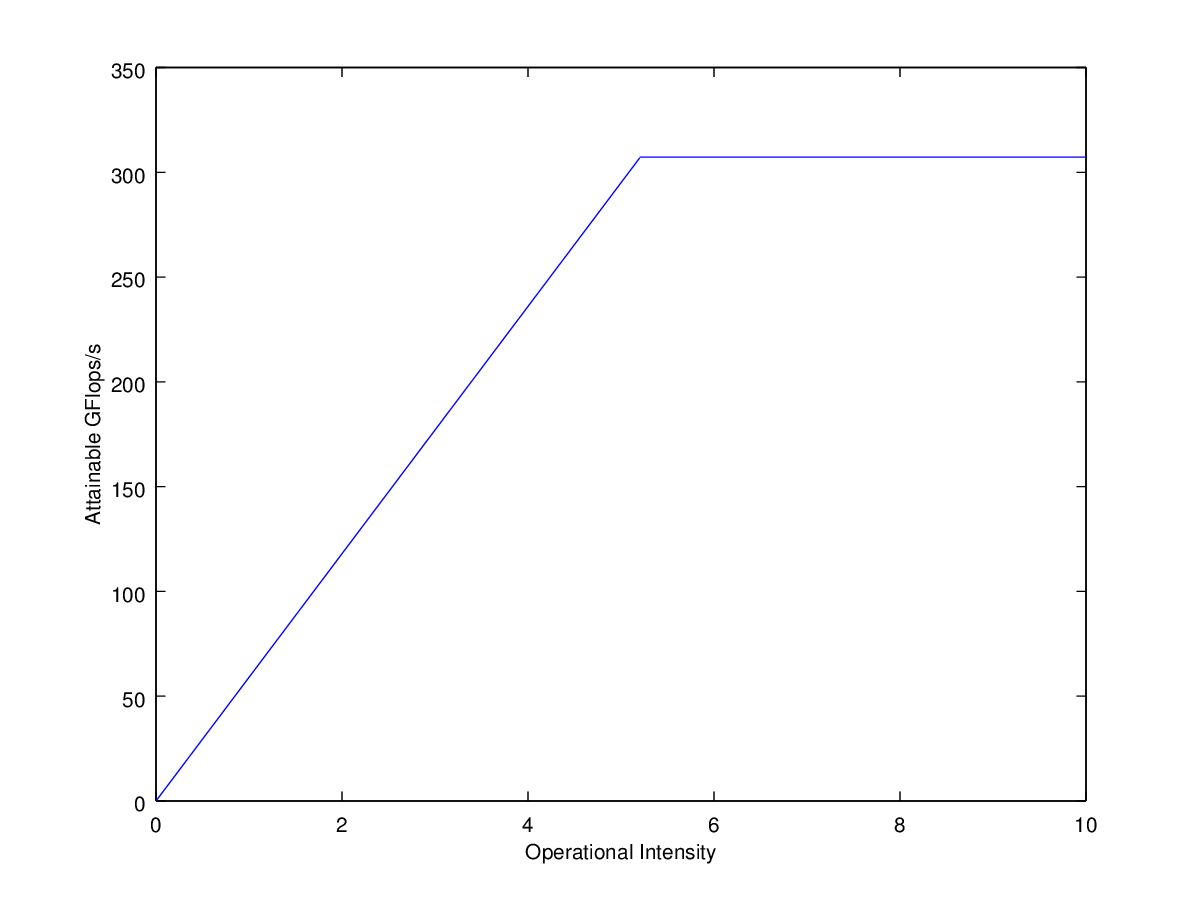
\includegraphics[width=5in]{q1.png}
        \end{figure}

        This changes when we have add 2 Phi boards because it changes our maximum possible GFlops per second. These 2 boards also have a different memory bandwidth (much higher than the compute nodes). Therefore depending on how the load was balanced over the compute node and two Phi boards, the plot would look different.

    \section*{Question 2}
        Two cores has two separate CPUs, one core with hyperthreading just schedules two threads onto the same CPU. On two cores, we can have more arithmetic operations going per unit time since we more ALUs. On one core, we only have one ALU, so we have half as many possible flops per cycle compared with two cores.

    \section*{Question 3}
        The Xeon Phi Coprocessor boards have an architecture look something like this: \\
        (http://www.transtec.co.uk/fileadmin/Medien/pdf/HPC/intel/intelxeonphi\_blockdiagram\_600.jpg):
        \begin{figure}[H]
            \centering
            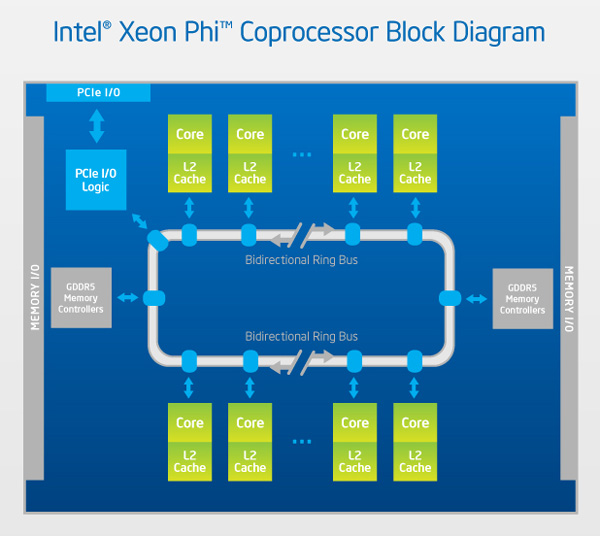
\includegraphics[width=5in]{q3.jpg}
        \end{figure}

        Each core has its own L1 and L2 cache, and all the cores are arranged in a ring connected by a directional bus. Located on either side of the ring, we have two memory controllers that access main memory, pass the data along the bus so that the cores can get the memory. Therefore, memory access is non-uniform, since the cores closer to the memory controllers will have access to the data first.

    \section*{Question 4}
        The dot product implementations result in each processor computing a sum and sending that to another processor. This results in a tree of depth $\log_2 n$ of nodes performing the summation operation, where $n$ is the number of processors. However, we have to send a message every time we have to compute a sum. So, if we do all the messaging in parallel, we need to send at least 1 message per level. Suppose it takes time $t$ to send 1 message. On the bottom most level, we need to perform $\frac{2m}{n}$ floating point operations per core, where $m$ is the number of elements in the vector. Therefore, if $n = 1$, we need to perform $2m$ floating point operations. Suppose $2m$ floating point operations takes time $\tau$, we then have the following relation for speed up when $n < m$:
        \begin{align*}
            S(n) = \frac{\tau}{\frac{\tau}{n} + t(\log_2(n))}
        \end{align*}

        When $n >= m$, we are limited by the number of elements in the vector, so $S(n)$ becomes constant with respect to $n$:
        \begin{align*}
            S(n) = \frac{\tau}{\frac{\tau}{m} + t(\log_2(m))}
        \end{align*}

\end{document}